\documentclass{aes2e}

% Metadata Information
\jyear{2016}
\jmonth{January}
\jvol{1}
\jnum{1}

\usepackage{color,url}
\newcommand{\gl}[1]{\textcolor{red}{gl: #1}}
\newcommand{\mr}[1]{\textcolor{green}{Mathias : #1}}
\newcommand{\ml}[2][]{\textcolor{blue}{#1 #2}}
\newcommand{\nm}[1]{\textcolor{magenta}{nm: #1}}
%\renewcommand{\baselinestretch}{2}

\begin{document}
%
% --- Author Metadata here ---
%\CopyrightYear{2007} % Allows default copyright year (20XX) to be over-ridden - IF NEED BE.
%\crdata{0-12345-67-8/90/01}  % Allows default copyright data (0-89791-88-6/97/05) to be over-ridden - IF NEED BE.
% --- End of Author Metadata ---

\title{Semantic browsing of sound databases \\ without keywords}
%\subtitle{[Extended Abstract]
%\titlenote{A full version of this paper is available as
%\textit{Author's Guide to Preparing ACM SIG Proceedings Using
%\LaTeX$2_\epsilon$\ and BibTeX} at
%\texttt{www.acm.org/eaddress.htm}}}
%strain
% You need the command \numberofauthors to handle the 'placement
% and alignment' of the authors beneath the title.
%
% For aesthetic reasons, we recommend 'three authors at a time'
% i.e. three 'name/affiliation blocks' be placed beneath the title.
%
% NOTE: You are NOT restricted in how many 'rows' of
% "name/affiliations" may appear. We just ask that you restrict
% the number of 'columns' to three.
%
% Because of the available 'opening page real-estate'
% we ask you to refrain from putting more than six authors
% (two rows with three columns) beneath the article title.
% More than six makes the first-page appear very cluttered indeed.
%
% Use the \alignauthor commands to handle the names
% and affiliations for an 'aesthetic maximum' of six authors.
% Add names, affiliations, addresses for
% the seventh etc. author(s) as the argument for the
% \additionalauthors command.
% These 'additional authors' will be output/set for you
% without further effort on your part as the last section in
% the body of your article BEFORE References or any Appendices.

% of EIGHT authors. SIX appear on the 'first-page' (for formatting
% reasons) and the remaining two appear in the \additionalauthors section.
%

%Author Info.
\authorgroup{
\author{Gr\'egoire Lafay$^1$}, \author{Nicolas Misdariis$^2$},
\author{Mathieu Lagrange$^1$}, \author{Mathias Rossignol$^2$}
\email{(gregoire.lafay@irccyn.ec-nantes.fr)}
\affil{IRCCyN, Ecole Centrale de Nantes $^1$ \quad\quad\quad\quad STMS Ircam-CNRS-UPMC $^2$}
}  


% There's nothing stopping you putting the seventh, eighth, etc.
% author on the opening page (as the 'third row') but we ask,
% for aesthetic reasons that you place these 'additional authors'
% in the \additional authors block, viz.
%\additionalauthors{Additional authors: John Smith (The Th{\o}rv{\"a}ld Group,
%email: {\texttt{jsmith@affiliation.org}}) and Julius P.~Kumquat
%(The Kumquat Consortium, email: {\texttt{jpkumquat@consortium.net}}).}
\date{26 December 2014 }
% Just remember to make sure that the TOTAL number of authors
% is the number that will appear on the first page PLUS the
% number that will appear in the \additionalauthors section.

\maketitle

\begin{abstract}
~In this paper, we study the relevance of a semantic organization of sounds to ease the browsing of a sound database. For such a task, semantic access to data is traditionally implemented by a keyword selection process. However, various limitations of written language, such as word polysemy, ambiguities, or translation issues, may bias the browsing process.

We present and study the efficiency of two sound presentation strategies that organize sounds spatially so as to reflect an underlying semantic hierarchy. For the sake of comparison, we also consider a display whose spatial organization is only based on acoustic cues. Those three displays are evaluated in terms of search speed in a crowdsourcing experiment using two different corpora: the first is composed of environmental sounds from urban environments and the second of sounds produced by musical instruments. Coherent results achieved by considering the two different corpora demonstrate the usefulness of using an implicit semantic organization to display sounds, both in terms of search speed and of learning efficiency. 
\end{abstract}

\keywords{Audio content management and display, Semantic sound data mining}

\section{Introduction}

With the growing capability of recording and storage devices, the problem of indexing large audio databases has recently been the object of much attention \cite{Wold1996}. Most of that effort is dedicated to the automatic inference of indexing metadata from the actual audio recording \cite{Zhang1999, tzanetakis2002musical}; in contrast, the ability to browse such databases in an effective manner has been less considered.

Thus, most media asset management systems are based on keyword-driven queries. The user enters a word which best characterizes the desired item, and the interface presents him with items related to this word. The effectiveness of this principle is primarily based on the typological structure and nomenclature of the database. However, for sound databases, several issues arise:

\begin{enumerate}
\item Sounds, as many others things, can be described in many ways. Environmental sounds in particular may be designated by their
source (a car door),  the action of that source (the slamming of a car door) or their environment (slamming a car door in a garage) \cite{houix2012lexical, niessen2010categories, brown2011towards}. Designing an effective keyword-based search system requires an accurate description of each sound, which has to be suited to the sound representation of the user to be effective.
\item Pre-defined verbal descriptions of the sounds made available to the users may potentially bias their browsing and final selection.
\item Localization of the query interface is made difficult as the translation of some words referring to qualitative aspects of the sound, such as its ambiance, is notoriously ambiguous and subject to cultural specificities.
\item Unless considerable time and resources are invested into developing a multilingual interface, any system based on verbal descriptions can only be used with reduced performance by non-native speakers of the chosen language.
\end{enumerate}
To circumvent those issues, not relying on keywords is desirable. However, conveying semantics remains a necessity for ease of browsing, which raises the question of what alternate means, other than written language, can be used to that end.

We thus consider in this paper three means of displaying sounds without relying on any textual representation, all based on a spatial organization of sounds. The first one, considered as a reference baseline, does not rely on any semantic information and positions sounds according to their acoustical properties (time averaged spectral features). The second and third displays exhibit a spatial organization based  on a predefined hierarchical semantic organization; those last two displays differs by how semantics are used.

Their effectiveness is studied through a search-based task whose aim is to find a given target sound by browsing the database using the display under evaluation. Two corpora are considered for this study: the first one is composed of sounds recorded in a urban environment, and the second of sounds produced by musical instruments.

The paper is organized as follows: in Section~\ref{previous}, previous work on the topic of sound database browsing is reviewed. The two corpora used in this study are then introduced in Section~\ref{dataset}. The three displays under evaluation are next described in Section~\ref{display}, and the crowdsourcing test used to compare them using the two different corpora is presented in Section~\ref{test}. The outcomes of those experiments are discussed in Sections~\ref{resultsu} and ~\ref{resultsm}.

\section{Previous work} \label{previous}



\begin{figure}[t]
\begin{center}
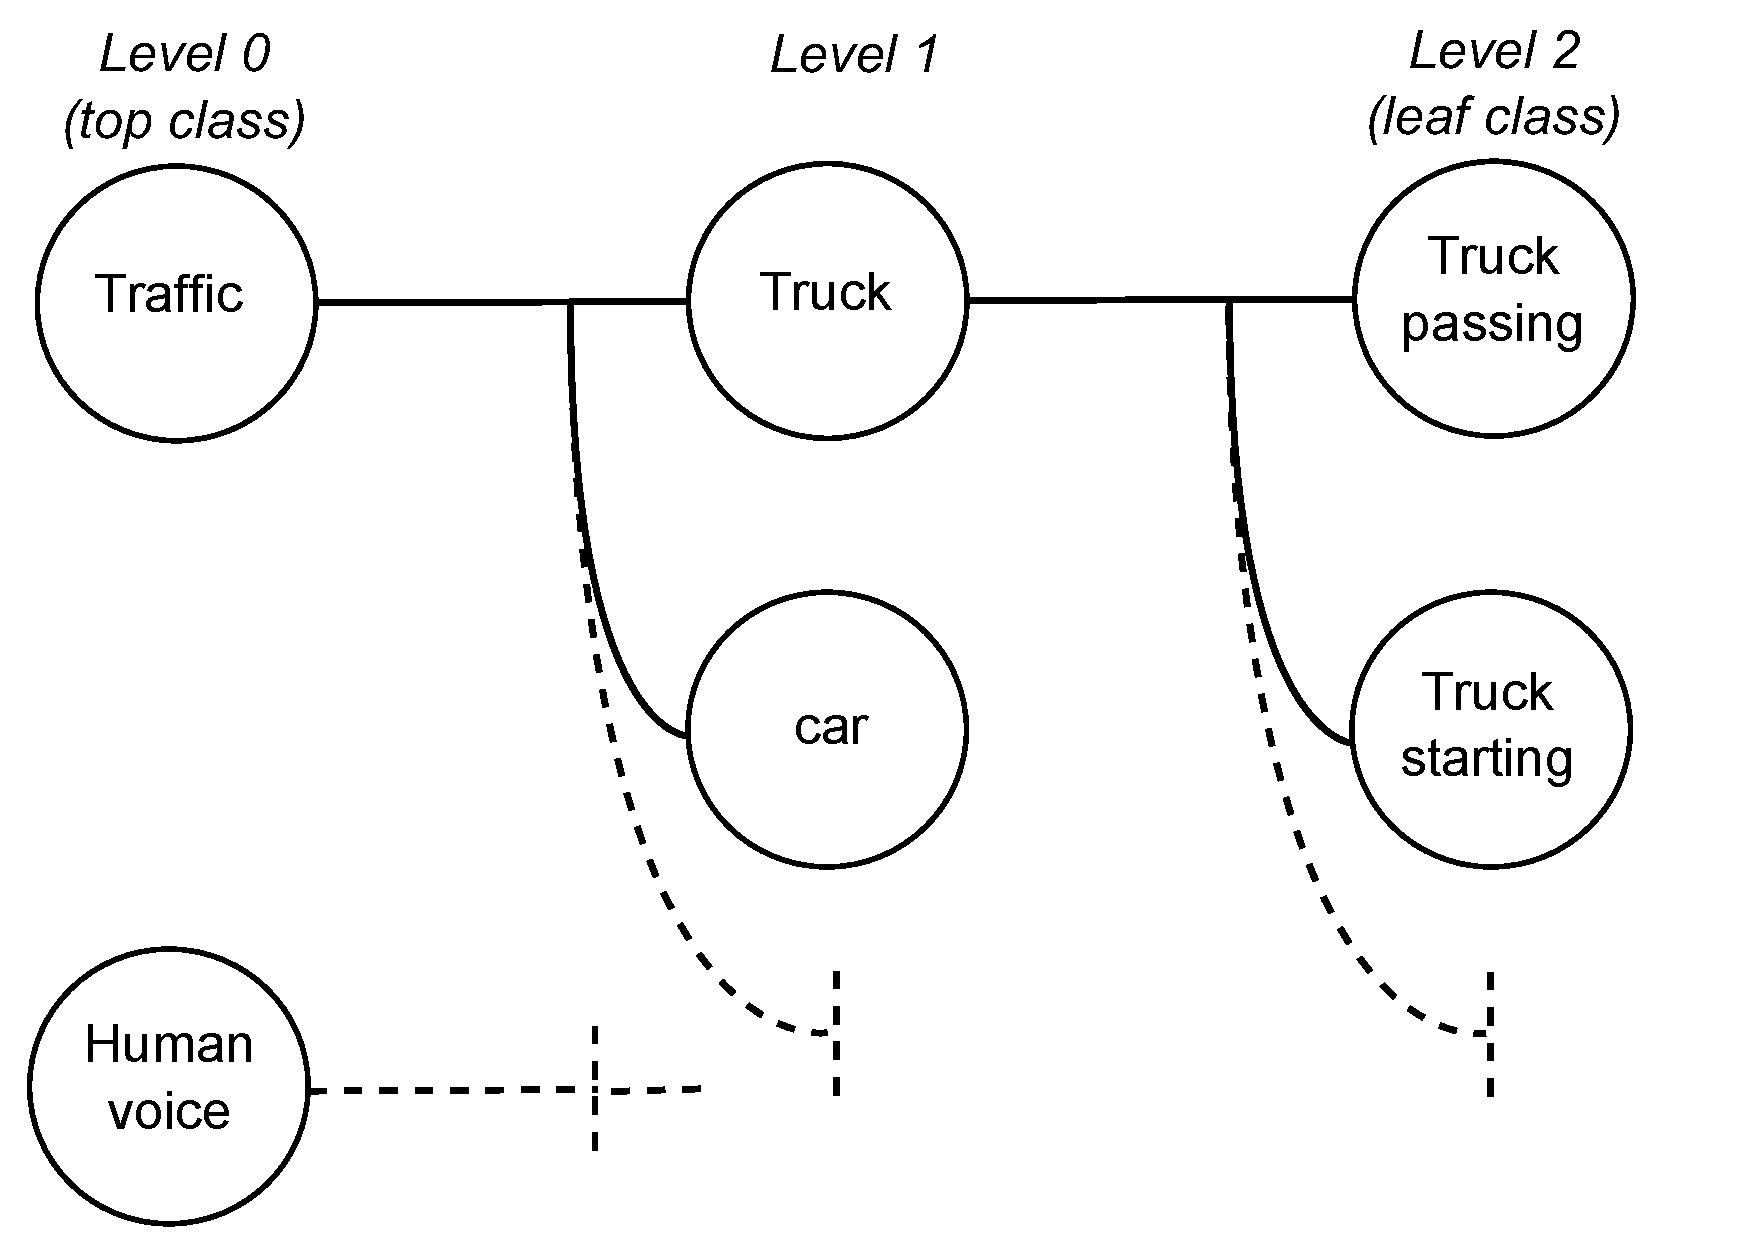
\includegraphics[scale=0.24]{gfx/dataset.pdf} 
\end{center}
\caption{\label{figdataset} Semantic hierarchical structure of the dataset of urban environmental sounds.}
\end{figure}


Most of the research effort in the sound design and Music Information Retrieval (MIR) communities is focused on acoustical based indexing and browsing \cite{tzanetakis2003musescape, streich2008music,goto2005musicream,pampalk2007musicsun}. Typically, the items (sound effects or pieces of music) are modeled by processing the digital audio waveform through some signal processing pipeline in order to get a compact description of each item
\cite{coleman2007mused}, with sometimes additional textual features. Then, statistical projections or embedding techniques, like Principal Components Analysis (PCA) \cite{MusicBox},  Multi Dimensional Scaling (MDS) \cite{schwarz2009sound,Cano2002}, Self Organizing Maps (SOM) \cite{pampalk2004exploring,pampalk2006musicrainbow,knees2006innovative} and the like are used to project the items in a two or three dimensional space while preserving as much as possible the distances among them. One of the advantages of such an approach is its ability to scale to very large databases \cite{schwarz2009scalability} as it does not need any kind of manual annotation and allows the user to search by similarity efficiently according to acoustical properties.

However, acoustical models are inherently subject to observation noise and biases. Selecting the most relevant features to achieve the correct projection of the data may only be performed by an expert user, taking into account the specifities of the data. If done \textit{a priori} by an expert or by some above cited dimensionality reduction technique, the induced bias can strongly limit the users' ability to access what they search for. In that respect, semantic tags, if available, have the advantage of implicitly structuring the similarity space, thus possibly easing the browsing process even if the actual tags are not -- as in this study -- explicitly exposed to the user.

\section{Datasets} \label{dataset}



The datasets considered in this study are respectively composed of 149 urban environmental sound events and 137 sounds produced by musical instruments. 

In the first corpus, a sound is characterized by a tag describing the physical source of the sound (\textit{man-yelling}, \textit{car-passing}). Sounds are then hierarchically grouped into classes according to their tags (\textit{car} $>$ \textit{car-passing}; \textit{car} $>$ \textit{car-starting}). Those classes are in turn packed into classes until high level classes describing broader concepts are reached (\textit{traffic} $>$ \textit{car} $>$ \textit{car-passing}). The sound dataset is thus organized into a hierarchical structure of semantic classes as described in Figure~\ref{figdataset}, where the sound samples of the dataset are the leaf semantic levels. All the other classes are represented by a \textit{prototype sound} that best characterizes the sounds belonging to the class. 

In order for the semantic hierarchical structure to be perceptually valid, the \textit{tags} that describe the classes  are chosen from sound categories presented in studies addressing environmental auditory scenes perception \cite{niessen2010categories, brown2011towards, dubois2006cognitive}. In cognitive psychology, sound categories may be regarded as intermediaries between collective sound representations and individual sensory experiences \cite{dubois2006cognitive}. It is our belief that using such category names to build the hierarchical structure makes it perceptually motivated, and can thus help the users to efficiently browse the dataset.

Similarly, the second corpus also has a semantic organization: high and mid level classes categorize musical instruments according to the means by which sound is produced, while leaf level classes are related to specific instruments (\textit{string} $>$ \textit{plucked-string} $>$ \textit{viola}; \textit{brass} $>$ \textit{ordinario} $>$ \textit{trumpet}).


\begin{figure}[t]
\begin{center}
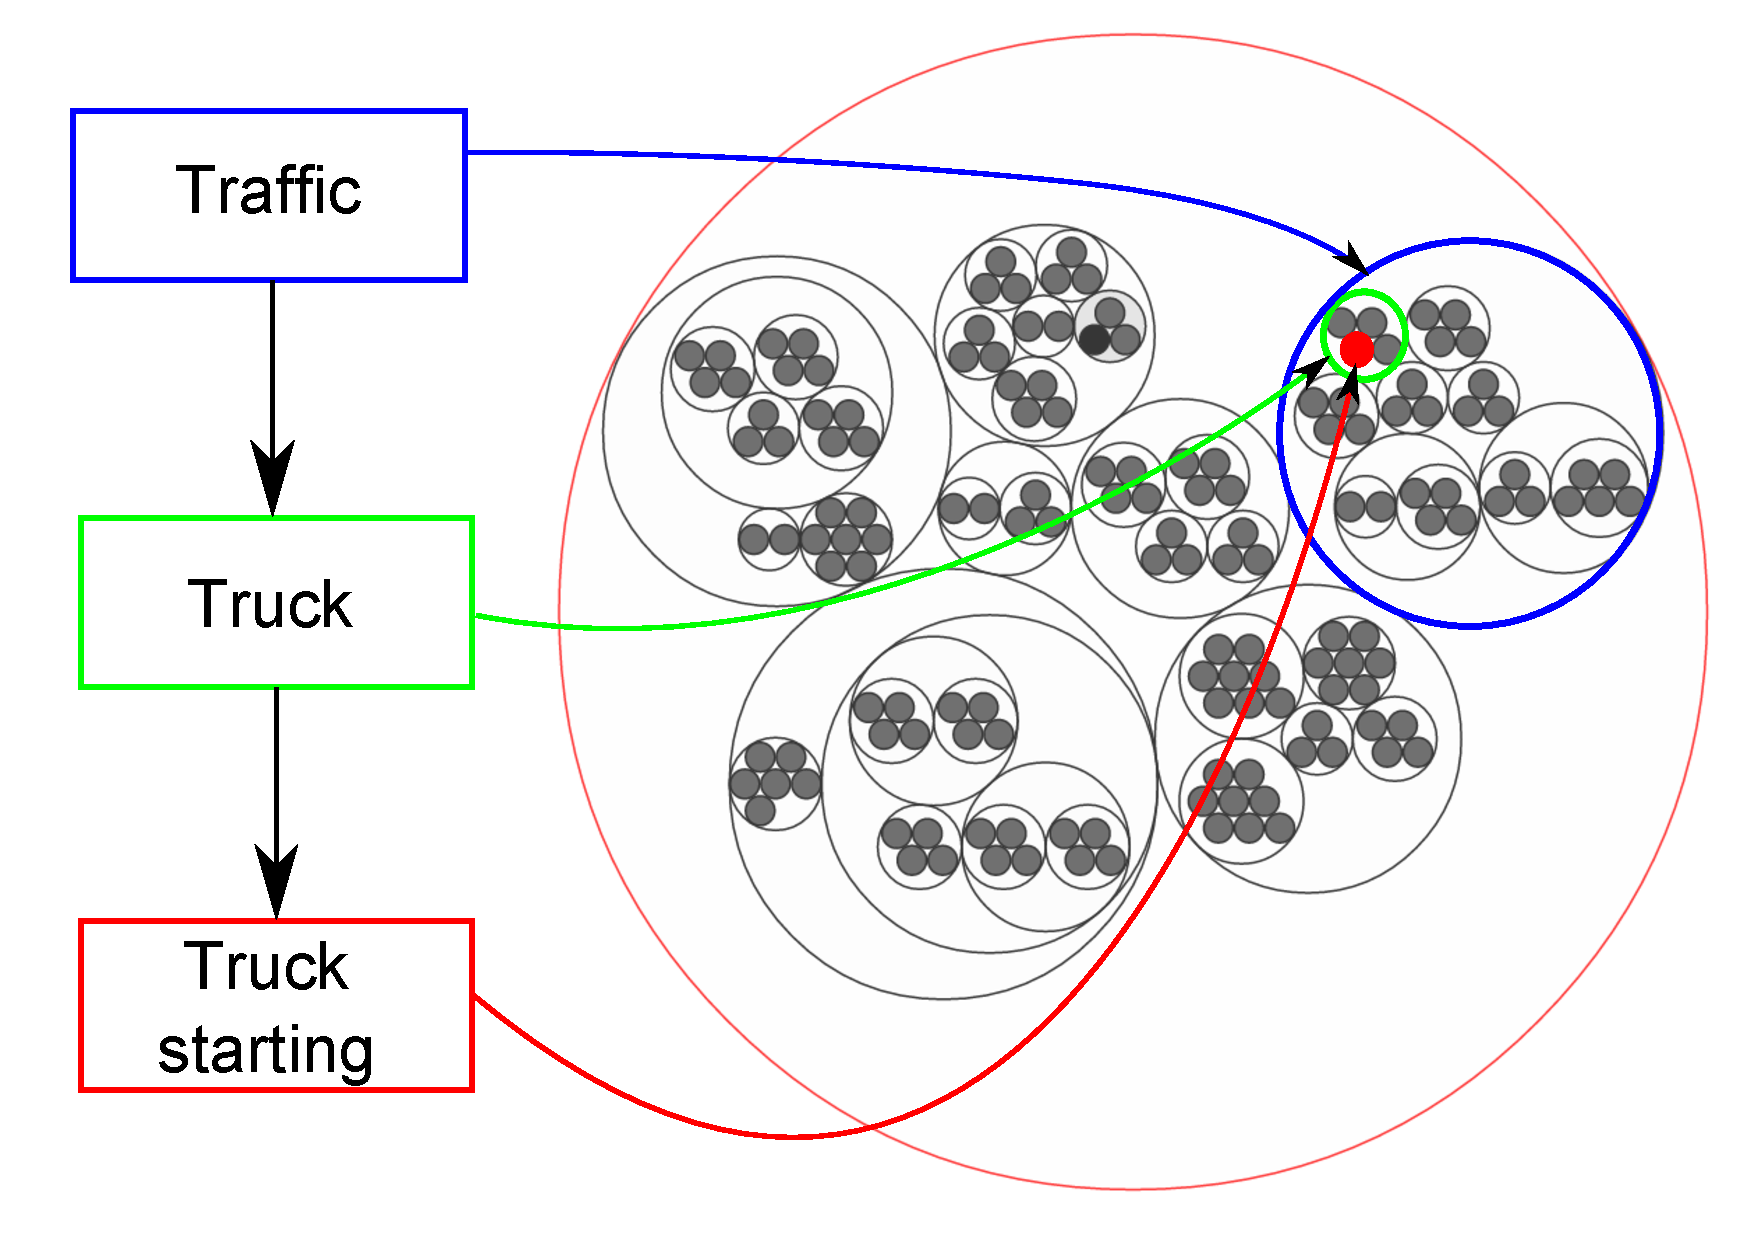
\includegraphics[scale=0.24]{gfx/SSF.pdf} 
\end{center}
\caption{\label{figSSF} Semantic displays are  based on the semantic hierarchical structure of the dataset.}
\end{figure}

%We choose to represent each sound leaf class of our sound data set with a circle. Circles are dispatched in a 2D space and packed together according to the hierarchical structure of the sound set (see figure \ref{SSF}). The class is identified by listening to an acoustic prototype chosen by the authors for its representativeness. Clicking on a circle fires this audio prototype.

\section{Displays} \label{display}

The aim of the displays described in this section is to allow the user to efficiently browse the sound datasets without any written textual help. In all displays, each sound is graphically represented by a filled circle which, once clicked, plays the actual sound. The spatial organization of circles is specific to each display.

As a reference, an Acoustic Display (AD) provides a spatial representation based on acoustic descriptors. Each sound is described by time-averaged Mel-Frequency Cepstrum Coefficients (MFCCs) computed with standard parameter settings (13 lowest quefrency coefficients are kept out of 40). The Euclidean distance between time averaged features is then computed for each sound pair. A non metric multidimensional scaling (MDS) with Kruskal's normalized stress \cite{kruskal1964multidimensional} is then employed to project the data into two dimensions according to this distance, as shown on Figure~\ref{figXP3music}. The latter exhibit a clear distinction between percussive (left) and sustained sounds (right).

% s~\ref{figXP3urban} and

Among the several alternatives that exists, MFCCs features are chosen as they are widely used in the audio processing community. MDS is selected for 2D projection as it has a lower sensitivity to outliers than the PCA and do not relyi on any parameter optimization, unlike the SOM approach. 

%\begin{figure}[t]
%\begin{center}
%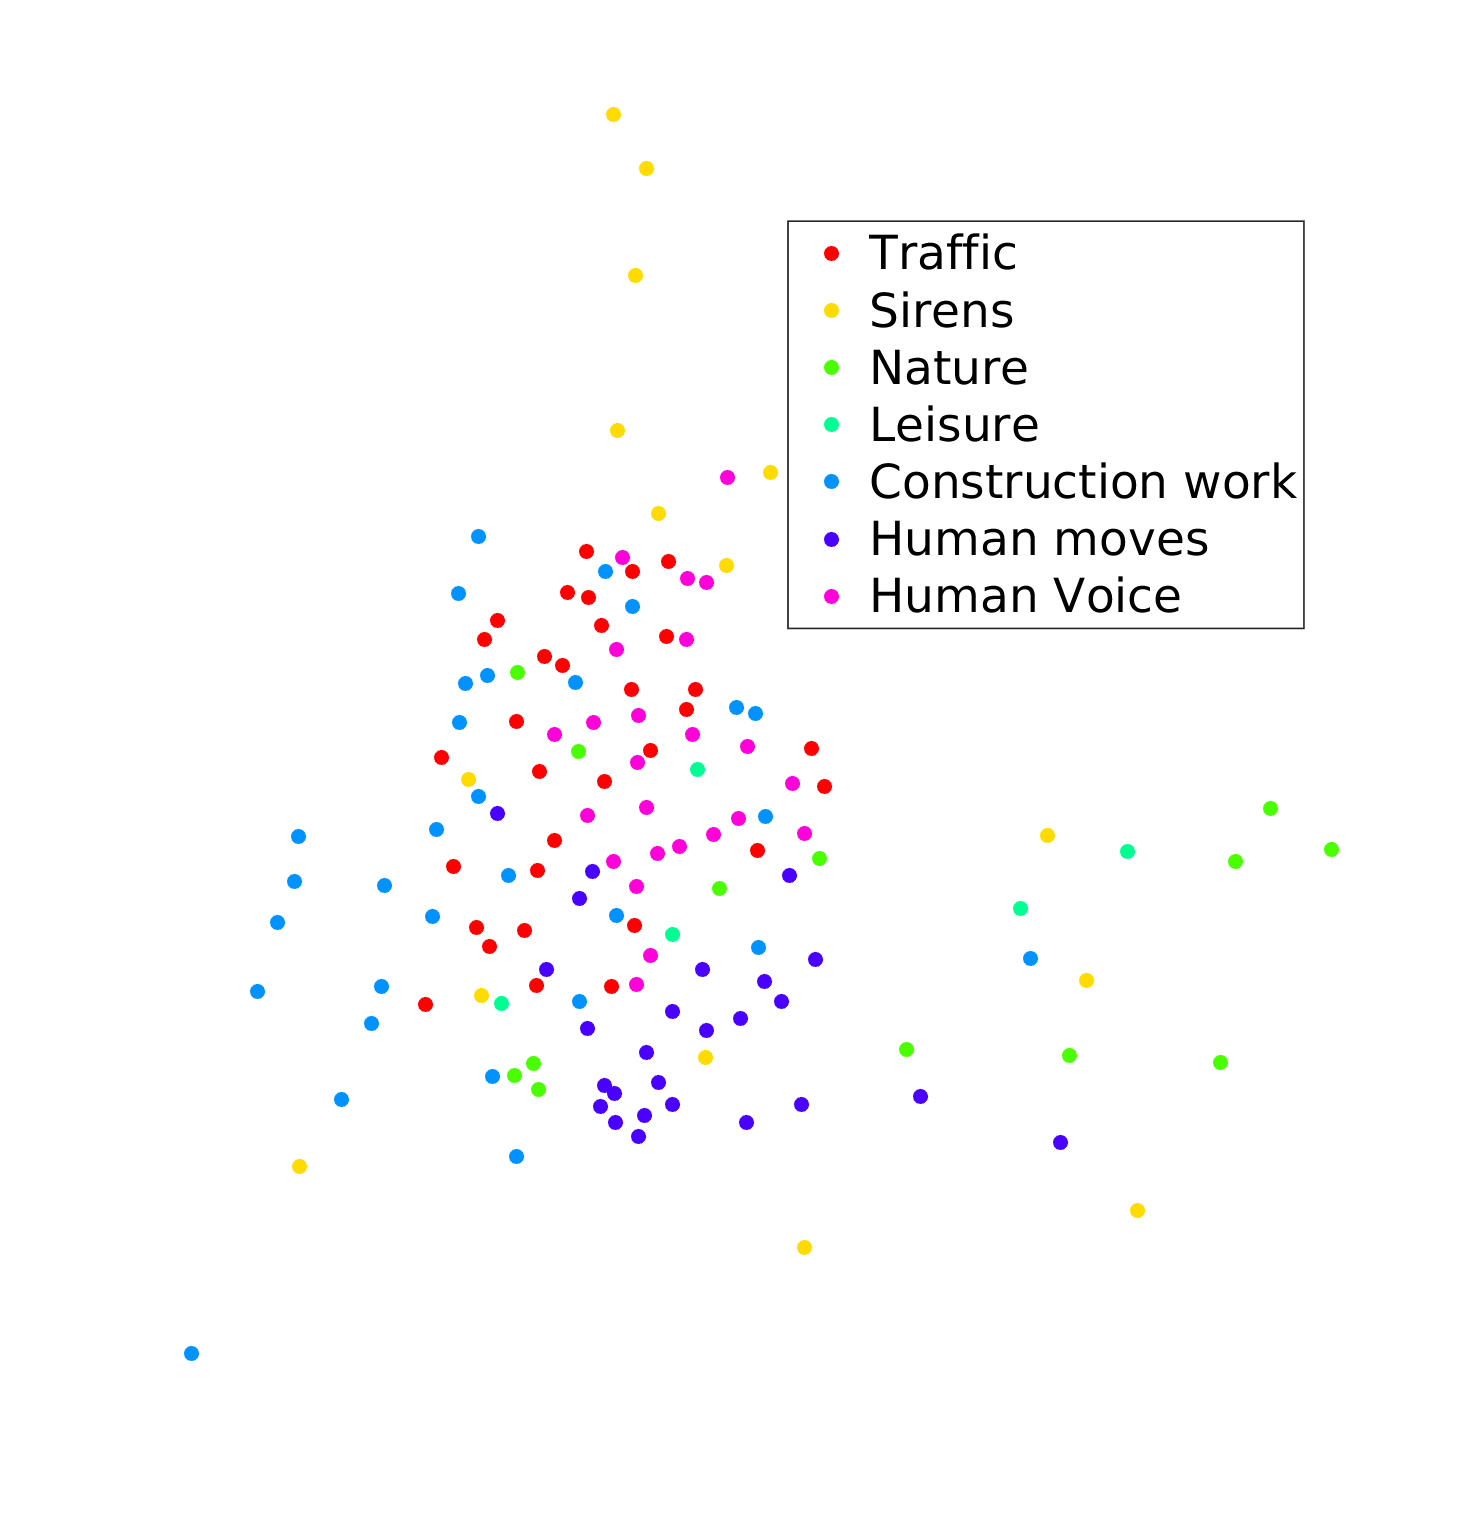
\includegraphics[width=\columnwidth]{gfx/urban_mds.png} 
%\end{center}
%\caption{\label{figXP3urban} Acoustical Display for the urban sound dataset (AD). Colors and legend are removed during the experiment.}
%\end{figure}

\begin{figure}[t]
\begin{center}
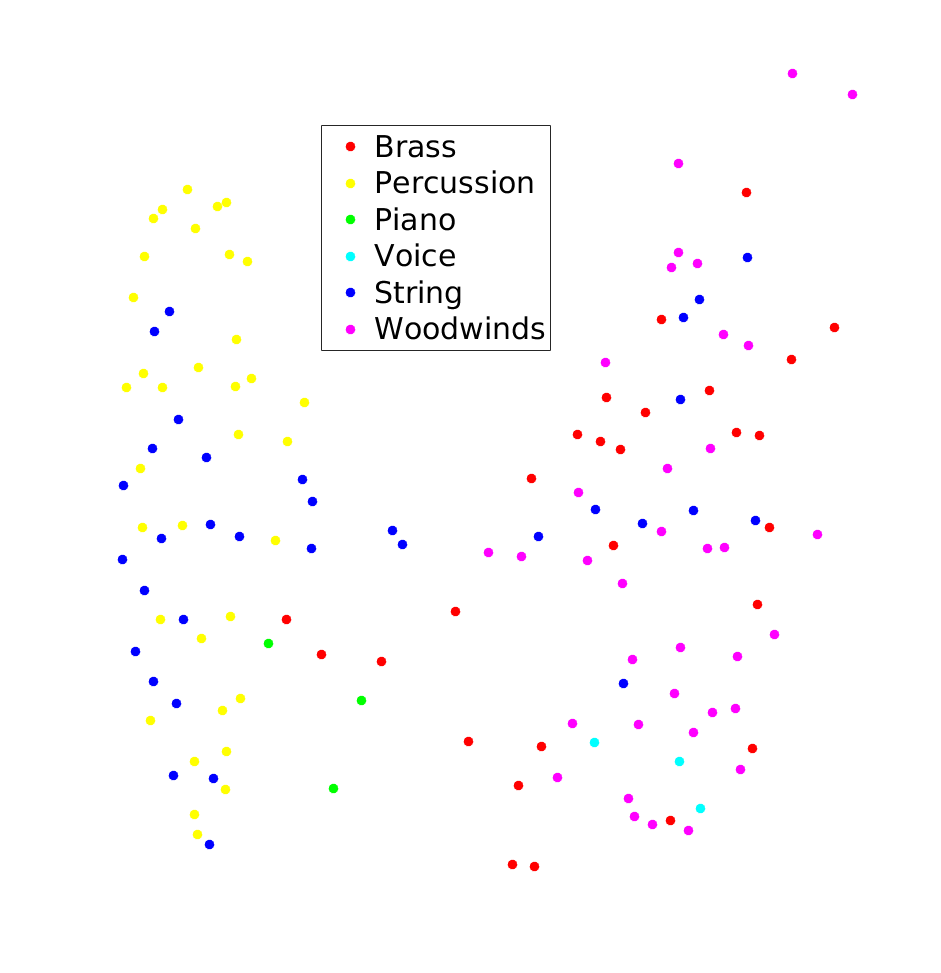
\includegraphics[width=\columnwidth]{gfx/music_mds.png} 
\end{center}
\caption{\label{figXP3music} Acoustical Display for the musical sound dataset (AD). Colors and legend are removed during the experiment.}
\end{figure}

Two semantically oriented displays are then proposed, called Full Semantic Display (FSD) and Progressive Semantic Display (PSD). Both display  consider the hierarchical structure of the dataset to organize sounds. Each sound class is represented by a filled circle. Circles are then packed together according to the hierarchical semantic organization of the dataset, as shown in Figure~\ref{figSSF}. Thus, subclasses belonging to the same class are close to each others. Circle packing functions of the D3.js (Data-Driven Documents) javascript library \cite{2011-d3} are used to distribute the sound classes in the space. Depending on the display, the user can either access each leaf class directly (FSD), or has to click through intermediate levels of the hierarchy (PSD). 

More precisely, with the FSD display, users can directly visualize the whole hierarchy, down to the leaf classes, while with the PSD display, users only have access, at first, to the intermediate semantic levels of the hierarchy. Upon first using PSD, they observe circles representing the top classes of the semantic hierarchical structure of the dataset. When users click on a circle, they hear the sound prototype of the class and the subclasses are progressively revealed, represented by white circles contained in the circle that has just been clicked. The same action is repeated until the user reaches the leaf classes of the hierarchy. The leaf classes are represented with small gray circles, indicating that there is no subclass to uncover. Thus the PSD has a constrained exploration system. Each time a sub-circle is automatically revealed, its sound prototype is played. Users may stop the discovery process by clicking on an other circle. In this display, the leaf classes are distributed  in the same manner as FSD. Thus, the spatial configuration of the unfolded version of PSD, which may be obtained after discovering all the classes and subclasses, is identical to the one of FSD.

%\mr{À enlever si vous êtes d'accord, c'est répété juste en-dessous : The PSD interface is introduced in order to study if a progressive top-down display of the hierarchical structure helps the user explore and understand the dataset hierarchy.}

\section{Experiments} \label{test}

\subsection{Objective}

During this experiment, the three displays are compared using two corpora: the urban sound corpus and the musical sound corpus. By comparing AD and xSD (the two semantic displays), the goal is to evaluate the  relative efficiencies of semantic based and acoustic based spatial configurations. By comparing FSD and PSD, we study the impact of an enforced hierarchical exploration of the corpus by the user. The goal is to check if constraining the user to first browse the high levels of the hierarchy helps him to grasp and memorize the spatial configuration and the organization of the sound classes. 

\subsection{Experimental protocol}

We evaluate and compare those three displays with a crowdsourcing web-based experiment\footnote{The tests are available at \url{http://soundthings.org/research/speedSoundFinding/index.html} and \url{http://soundthings.org/research/speedSoundFindingMusic/index.html}, each of the 3 displays is also available by appending a digit from 1 to 3 to \textit{index} in the above cited url.} for which we adopt a between subject approach, \textit{i.e.} a subject can only test one display. In this experiment, subjects are asked to successively retrieve 13 target sounds among the whole dataset. The target sounds are selected such that there are at least two target sounds in each top-level class of the semantic hierarchical structure of the dataset. To reduce order effects, target sounds are presented to each subject in a random order.

First, the subject clicks a button to listen to the target sound. They may then replay the target sound as many times as they like, even while browsing. A timer starts when the subject clicks on a circle for the first time. When the target sound is found, the subject puts an end to the search by clicking on the \textit{Click if found} button. This action 1) stops the timer and 2) loads a new target sound. If the subject designates an incorrect sound, an error message appears, and the experiment goes on with the same target sound.

% MR : S'il y a besoin de gagner de la place, retirer le paragraphe suivant, ça n'apporte pas grand chose

%During the experiment, two visual cues are shown to the subject:
%\begin{itemize}
%\item \textit{The search state}: which can be "pause" if the subject is not currently looking for a target sound (at the beginning of the experiment, or between two target sounds) or  "in progress"  if they are.
%\item \textit{Remaining target sounds}: the number of target sounds that remain to be found.
%\end{itemize}

The experiment ends when all the target sounds have been found. An important feature of the PSD display is that it is not reinitialized at each change of target sound. Thus, when a circle is unfolded, its content remains visible during the whole experiment.

\subsection{Data Collection}
Four types of data are collected during the experiment:
\begin{itemize}
\item the \textit{absolute duration}, which is the total duration of the entire experiment, including breaks between two target sound searches;
\item the duration of each search. The sum of the 13 search durations, which is the \textit{absolute duration} minus the break times between two target sound searches, is called the \textit{total search duration};
\item the name of each sound which has been listened to (from which the number of heard sounds can be deduced);
\item the time at which each sound has been heard.  
\end{itemize}

\subsection{Apparatus}

A crowdsourcing approach is adopted. 
%The experiment is designed to be performed using the \textit{Chrome} web browser. The link to the experiment has been sent to three  mailing lists, namely \textit{Music-Ir}, \textit{Auditory} and an internal IRCAM mailing list. 
Subjects are recruited using research mailing list and are only allowed to perform the experiment once, and on one interface only. % Data were automatically collected server-side at the end of the experiments. Subjects were asked to use headphones. 
All sounds of the dataset are normalized to the same root mean square (RMS) level.

% Je ne pense pas utile de préciser la technique utilisée pour empêcher les gens de faire l'expé deux fois, parce que (1) ce n'est pas fondamental, et (2) la technique est loin d'être parfaite.

\subsection{Participants}

60 subjects have completed the experiment for the urban sound dataset, 20 for each interface. 48 subjects have completed the experiment for the urban sound dataset: 17 for the PSD interface, 16 for the FSD interface and 15 for the AD interface.

\subsection{Outliers Detection}

Outlier detection is an important step of any crowdsourcing experiment as experimenters do not control the environment in which the subjects perform the experiment \cite{komarov2013crowdsourcing,buchholz2011crowdsourcing}. A commonly used method to detect outliers in  human-computer interaction studies is to consider as outlier an observation which deviates of at least $\pm2$ standard deviation from the average \cite{komarov2013crowdsourcing}. However, as this latter method is not robust to the presence of isolated extreme observations (as it is often the case for crowdsourcing experiment), we follow the  method proposed by \cite{komarov2013crowdsourcing} and use the Inter-Quartile Range ($IQR$). With this approach, an observation is considered to be an outlier if its value is more than $3*IQR$ higher than the third quartile or more than $3*IQR$ less than the first quartile. This methods is applied in this study to the four following criteria :

\begin{enumerate}
\item the \textit{absolute duration}: to detect subjects who took abnormally long breaks between searches;
\item the \textit{total search duration}: to detect subjects who spent an abnormally long time to complete the experiment;
\item number of heard sounds: to detect subjects who had to hear an abnormally high number of sounds to complete the experiment;
\item the maximum number of times a target sound had to be heard before being found: to detect subjects who had difficulty to recognize the target sounds.
\end{enumerate}

\subsection{Statistical analysis}

We use one-way ANOVA to test for statistical significance. Post hoc analyses are done using two samples \textit{t} tests with Bonferroni correction. All statistical analyses are performed at the 5\% significance level.


\section{Results on Urban Sounds} \label{resultsu}

\subsection{Outliers}

Using the $IQR$ method, 5 subjects are detected as outliers for the urban experiment, and removed from the analysis. 2 of those subjects used PSD and 3 used AD. 3 subjects are detected by considering the \textit{absolute duration}; they spent respectively 50 minutes, 5 hours and 17.5 hours to complete the experiment. One subject is detected by considering the \textit{total search duration} (46 minutes), and another by observing the \textit{total number of heard sounds} (1800 heard sounds, roughly 12 times the total size of the corpus). Lastly, 2 subjects are detected by observing the maximum number of times they had to hear a target sound before finding it (4 and 8 times). It should be noted that some subjects met several of the criteria.

\begin{figure}[t]
\begin{center}
\includegraphics[width=\columnwidth]{gfx/urbanMusic1.eps} 
\end{center}
\caption{\label{urbanMusic} Average and standard deviation for (a,d) the total search durations, (b,e) the number of heard sounds and (c,f) the number of unique heard sounds; considering respectively the urban dataset (a,b,c) and the music dataset (d,e,f).}
\end{figure}  

\begin{figure}[t]
\begin{center}
\includegraphics[width=\columnwidth]{gfx/analyse_urban2.eps} 
\end{center}
\caption{\label{fig2urban} Evolution of (a) the average search durations, (b) the average numbers of heard sounds, and (c) the average numbers of unique heard sounds at each target sound search, considering the urban dataset. Lines are linear regression fits.}
\end{figure}


\begin{figure}[t]
\begin{center}
\includegraphics[width=\columnwidth]{gfx/analyse_music2.eps} 
\end{center}
\caption{\label{fig2Music} Evolution of (a) the average search durations, (b) the average numbers of heard sounds, and (c) the average numbers of unique heard sounds at each target sound search, considering the music dataset. Lines are linear regression fits.}
\end{figure}

\subsection{Efficiency}

To study the relative efficiency of the three displays, three metrics are considered: 

\begin{itemize}
\item the \textit{total search duration},
\item the number of heard sounds during the whole experiment,
\item the number of unique sounds heard during the whole experiment. By "unique" we mean that, if a same sound is heard 10 times during the 13 searches of the  experiment, it counts only for one. 
\end{itemize}

The first two metrics quantify the notion of efficiency by considering the time and the number of clicks needed to achieve the task, \textit{ie.} reach the target. The goal for those values is to be as low as possible. The third data allows us to measure the selectivity of the interfaces. A low number of unique heard sounds indicates that subjects understood the spatial organisation of the dataset, and used this knowledge to improve their searches. On the contrary, a high number of heard sounds without duplication suggests that the subject did not understand the way sounds are organized in space, and tended to play all the sounds at each search. The maximum number of unique heard sounds is the corpus size: 149 sounds.

The averages and standard deviations for the three metrics are presented in Figure~\ref{urbanMusic}. The type of display has a significant effect on the the \textit{total search duration} ($F[2,52]=4; p<0.05$), the number of heard sounds ($F[2,52]=6; p<0.01$) and the number of unique heard sounds ($F[2,52]=9; p<0.01$). 

Post hoc analysis on the total search duration (Figure~\ref{urbanMusic}.a) shows no significant differences between the three interfaces (PSD-FSD: $p=0.09$; PSD-AD: $p=1$; FSD-AD: $p=0.07$), although the FSD interface achieves the best results.

Concerning the numbers of heard sounds (Figure~\ref{urbanMusic}.b), FSD significantly outperforms the AD interface (FSD-AD: $p<0.01$),  whereas PSD and FSD as well as PSD and AD show similar outcomes (PSD-FSD: $p=0.06$; PSD-AD: $p=1$).

Figure~\ref{urbanMusic}.c shows the results for the number of unique heard sounds. This time the results of AD are significantly higher (indicating an inferior performance) than those of both PSD and FSD (PSD-AD: $p<0.01$; FSD-AD: $p<0.01$).  For AD, 75\% of the subjects heard more than 140 sounds, and 25\% heard at least 148 sounds, that is almost the entire database. Considering PSD, 75\% of the subjects heard less than 134 sounds, versus 143 for FSD. This time PSD and FSD perform equivalently (PSD-FSD: $p=1$).

According to those results, a spatial display following a hierarchical organization of the dataset based on semantic values (PSD and FSD) is more efficient than an organization based on acoustic descriptors (AD) as it allows the users to quickly apprehend the dataset range and thus to specify their search. Furthermore the FSD interface allows the users to retrieve the 13 target sounds by listening to a smaller amount of sounds than the AD. However, those two effects are significantly compromised when users have to parse the entire hierarchy to reach the first target sound, as in the PSD display. It seems that enforcing an explicit exploration of the hierarchy disturbs or confuses the user instead of allowing him to learn the semantically motivated spatial organization of the classes. 


\subsection{Learning}

We now study if and how users progressively acquire knowledge about the spatial organization of the classes. To do that, the evolution of the above described metrics with respect to the search indexes is considered. Three sets of collected data are used:

\begin{itemize}
\item the duration of each target sound search,
\item the number of heard sounds for each target sound search,
\item the number of unique heard sounds for each target sound search. 
\end{itemize}

Figure~\ref{fig2urban}.a shows the evolution of the average duration of each target sound search observed for AD, FSD and PSD. As shown by a linear regression of the data, there is an overall increase of efficiency with respect to the index of the search. For the duration and the number of heard sounds (Figure~\ref{fig2urban}.b), AD and PSD perform equivalently, whereas FSD exhibits better performance. In the case of the number of unique heard sounds (Figure~\ref{fig2urban}.c), the two semantic displays are equivalent. This latter result suggests that for both semantic displays, users have parsed the same range of the dataset, although users of FSD have done so by listening to fewer sounds and more quickly. 

\section{Results on Musical Sounds} \label{resultsm}

\subsection{Outliers}

2 subjects are detected as outliers for the music experiment and removed from the analysis. 1 subject used PSD and 1 subject used FSD. The first outlier is detected by considering the \textit{absolute duration} (5 hours to complete the experiment) and the second by looking at the \textit{absolute duration} (1 hour and 30 minutes) as well as the \textit{total search duration} (1 hour and 15 minutes) and the total \textit{number of heard sounds} (901).

\subsection{Efficiency}

The averages and standard deviations for the three metrics are presented in Figure~\ref{urbanMusic}. The type of display has a significant effect on the the \textit{total search duration} ($F[2,43]=13; p<0.01$), the number of heard sounds ($F[2,43]=14; p<0.01$) and the number of unique heard sounds ($F[2,43]=5; p<0.05$).

Considering the \textit{total search duration} (Figure~\ref{urbanMusic}.d), post hoc analyses shows that PSD and FSD perform better than the AD interfaces (PSD-AD: $p<0.01$; FSD-AD: $p<0.01$;). No significant difference is found between PSD and FSD (PSD-FSD: $p=0.20$).

Figure~\ref{urbanMusic}.e shows the results for the numbers of heard sounds. This time AD and PSD exhibit similar results (PSD-AD: $p=0.19$), while being both outperformed by FSD (FSD-PSD: $p<0.01$; FSD-AD: $p<0.01$).

Considering the numbers of unique heard sounds (Figure~\ref{urbanMusic}.f), FSD significantly outperforms the AD interface (FSD-AD: $p<0.05$), while both PSD \emph{vs.} FSD and PSD \emph{vs.} AD show similar outcomes (PSD-FSD: $p=0.06$; PSD-AD: $p=1$). Those results confirms the trends observed for the urban sounds (see Section~\ref{resultsu}):

\begin{itemize}
\item A semantic organization of the dataset significantly reduces  the number of heard sounds needed to find a target sound.
\item Forcing the users to parse the entire hierarchical organization of the dataset seems to diminish the interface efficiency by increasing the number of sounds to be listened to.
\end{itemize}

PSD and FSD significantly reduce the search durations compared to an acoustic organization (AD), which was not the case for the urban sound dataset. This may be explained by the fact that the musical corpus has perhaps a more obvious semantic organization.

\subsection{Learning}

Figure~\ref{fig2Music} shows the evolution of the metrics with respect to the target sound index. Results for the music dataset are similar to those observed for the urban dataset. An overall increase of efficiency with respect to the index of the search is observed for the tree interfaces. For the duration and the number of heard sounds (Figure~\ref{fig2Music}.a and .b) the FSD interface exhibits better performance. Considering the number of unique heard sounds (Figure~\ref{fig2Music}.c), the learning of the dataset range seems to be quicker for the FSD interface than for the PSD interface. Once again, results show that enforcing the parsing of the hierarchy is not beneficial.

\section{Conclusion}

% \nm{Cela manque pt-etre d'une partie Discussion / Synthese ? Et la conclusion manque pt-etre un peu de perspectives : vers simScene, par exemple ?}
% MR : Cela manque peut-être, mais bon, 8 pages...

In this paper, two displays allowing users to explore a semantically organized sound dataset without written textual help are presented. The interfaces distribute sounds represented by circles on a 2D space, following an underlying hierarchical semantic organization. Those two semantic displays are assessed and compared to a third display in which the spatial configuration depends upon acoustic features. The tests consists in data retrieval tasks done using two different corpora. 
The Full Semantic Display (FSD), that allows users to directly visualize the leaf classes of the semantic hierarchical structure, proves to be the most effective interface for the task. This display has been integrated as a sound selector into a acoustic scene simulator that benefit from the advantages of such an approach: no need of localization and reduction of the potential bias of using description tags\footnote{\url{http://soundthings.org/research/urbanSoundScape/XP2014/simScene}}. 

Two main conclusions may be derived from this experiment. First, a spatial configuration based on semantic features is more effective to retrieve target sounds than a spatial configuration based on acoustic features. Second, imposing the exploration of the semantic hierarchical structure by constraining its visibility does not help the user understand and learn the spatial configuration of the semantic class, but instead disturbs the navigation. 

In the datasets considered in this study, there are as many leaf classes as sounds in the dataset, which would be unrealistic for larger datasets. In that case, the organization can easily be adapted by considering the leaf classes as \textit{collections} of semantically similar sound samples. Thus, two sounds of \textit{male-yelling} would be grouped into a single leaf class with the tag \textit{male-yelling}. The leaf class would then also have a \textit{prototype sound} being the most representative item of the different \textit{male-yelling} sounds belonging to the leaf class.

%It has to be noted that the test datasets are relatively small in terms of leaf sound classes. It may be interesting to test the FD on a larger dataset. 
%
%To conclude, if this study goal was to investigate the viability of an audio based data mining interface, other studies addressing comparison between FD and keyword based interfaces remain to be conducted. 


\section{Acknowledgements}

Research project partly funded by ANR-11-JS03-005-01.



\bibliographystyle{abbrv}
\bibliography{sigproc}  % sigproc.bib is the name of the Bibliography in this case


\biography{\textbf{Gr\'egoire Lafay}}{gfx/lafay.jpg}{IRCCYN, Ecole Centrale de Nantes, France}

\biography{\textbf{Nicolas Misdariis}}{gfx/lafay.jpg}{IRCAM, France}

\biography{\textbf{Mathieu Lagrange}}{gfx/lagrange.jpg}{IRCCYN, Ecole Centrale de Nantes, France}

\biography{\textbf{Mathias Rossignol}}{gfx/rossignol.jpg}{STMS Ircam-CNRS-UPMC, France}



%\begin{biography}[{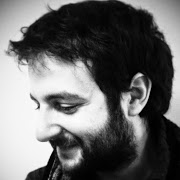
\includegraphics[width=1in,height=1.25in,clip,keepaspectratio]{gfx/lafay}}]{Gr\'egoire Lafay} was born in Paris, France, in 1990. He received in 2011 the B.S. degree in Acoustic from the University Pierre and Marie Curie (UPMC), Paris, France, and the B.S. degree in Musicology from the Sorbonne University, Paris, France. He received his M.S. degree in acoustics, signal processing and musical informatics (ATIAM) from the University Pierre and Marie Curie and the IRCAM laboratory, Paris, France, in 2013. Since 2013, he is a Ph.D student at Irccyn, a French laboratory dedicated to cybernetics. His current research interests include acoustic scene similarity and classification, as well as acoustic scene perception. 
%\end{biography}
%
%\begin{biography}[{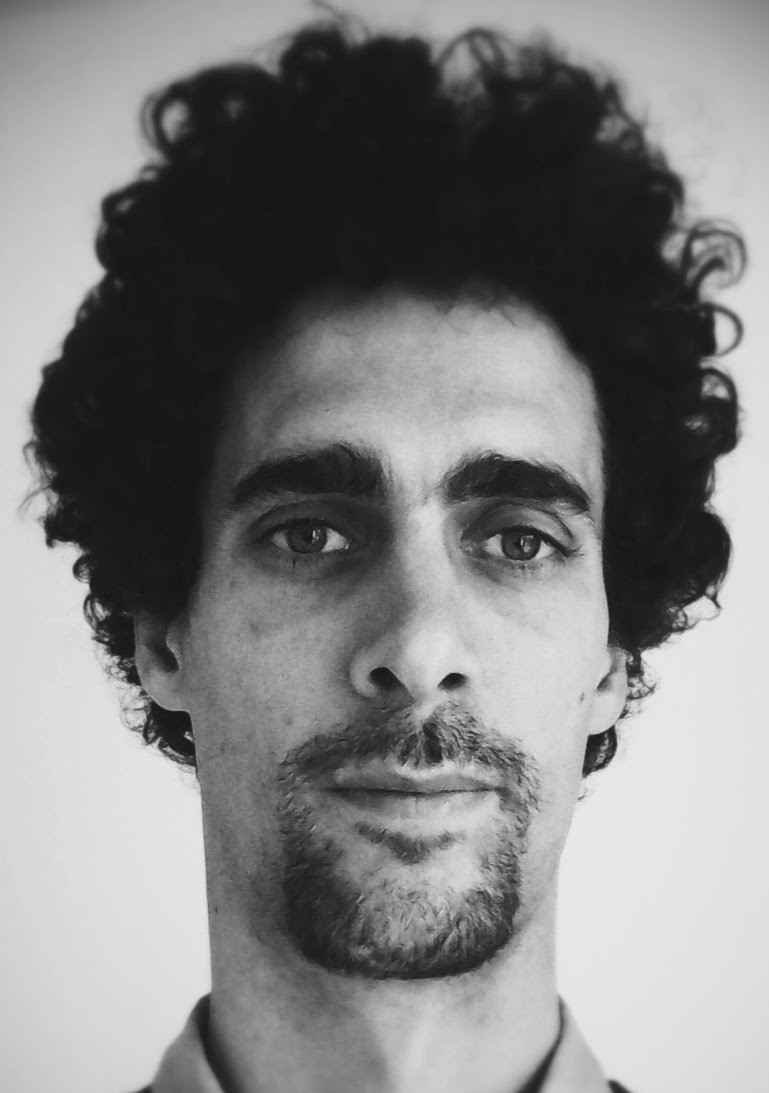
\includegraphics[width=1.25in,height=1.25in,clip,keepaspectratio]{gfx/lagrange}}]{Mathieu Lagrange} is a CNRS research scientist at Irccyn, a French laboratory dedicated to cybernetics. He obtained his PhD in computer science at the University of Bordeaux in 2004, and visited several institutions, in Canada (University of Victoria, McGill University) and in France (Orange Labs, Telecom ParisTech, Ircam). His research focuses on machine listening algorithms applied to the analysis of musical and environmental audio.
%\end{biography}
%
%\begin{biography}[{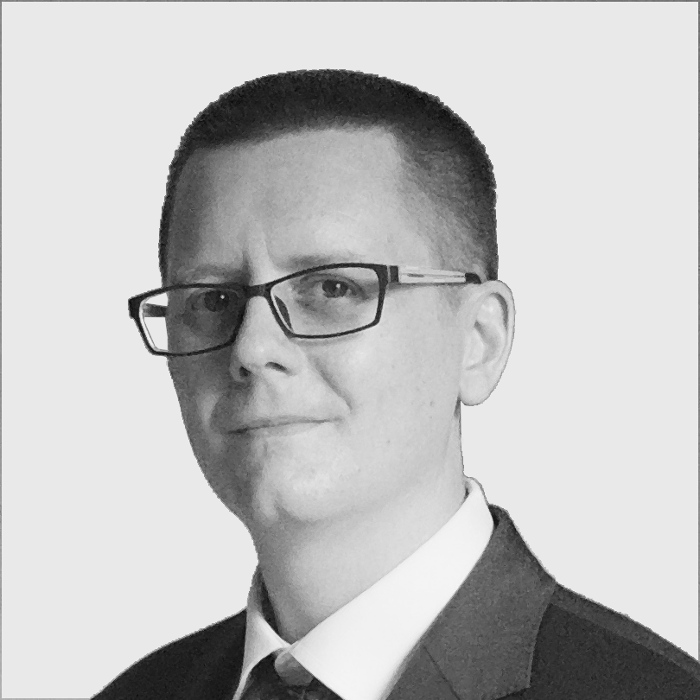
\includegraphics[width=1.05in,height=1.5in,clip,keepaspectratio]{gfx/rossignol}}]{Mathias Rossignol} obtained his PhD from Rennes University (France) in 2005, with a specialty in Natural Language Processing. He then focused his research on speech analysis and recognition at the International Research Center MICA (Hanoi, Vietnam), before moving on to Auditory Scene Analysis at IRCAM (Institute for Acoustic / Music Research and Coordination, Paris, France).
%\end{biography}
%
%\begin{biography}[{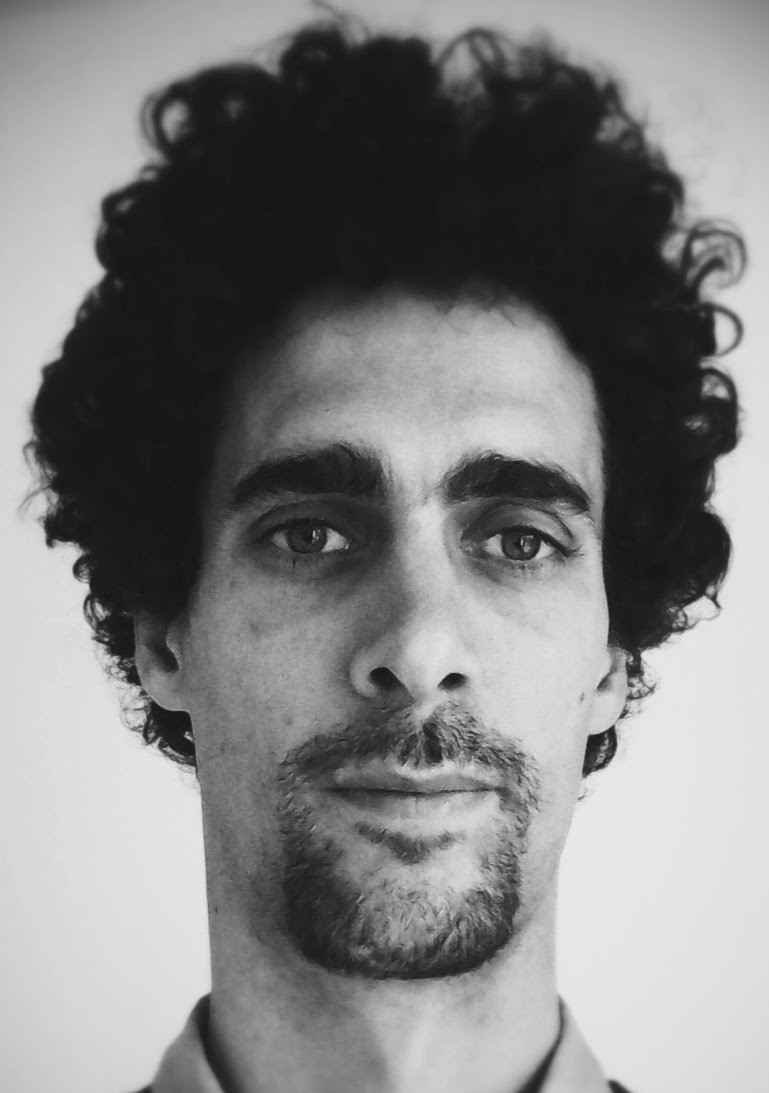
\includegraphics[width=0.9in,height=1.4in,clip,keepaspectratio]{gfx/lagrange.png}}]
%{Emmanouil Benetos} (S'09-M'12) received the B.Sc. and M.Sc. degrees in 
%informatics from the Aristotle University of Thessaloniki, Greece, in 
%2005 and 2007, respectively, and the Ph.D. degree in electronic 
%engineering from Queen Mary University of London, U.K., in 2012. From 
%2013 to 2015, he was a University Research Fellow with the Department of 
%Computer Science, City University London, London, U.K. He is currently a Royal 
%Academy of Engineering Research Fellow with the Centre for Digital Music, 
%Queen Mary University of London, U.K. His research focuses on signal 
%processing and machine learning for music and audio analysis, as well as 
%applications to music information retrieval, acoustic scene analysis, 
%and computational musicology.
%\end{biography}

%In particular, much consideration has been given in order to avoid any semantic bias. Indeed any selection process based on keyword searching would have influenced the subject choices, and makes impossible or inadvisable to run any kind of identification tasks. 
%
%In a previous study \cite{ssf} we found  that the perceptively inspired structured of the sound data set (on which depends the spatial configuration of the circles) offers a easy-to-navigate format that allows subject to quickly understand the spatial localization of the different sound element classes and thus  enable them to quickly find a sound after a short amount of time. 
%
%%The interface selection has been tested in a previous \textit{crowd-sourcing} experiment on 60 subject. The goal was to find 10 target sound. Results showed that this interface allows subject to learn the sound spatial organisation, and to quickly retrieve a sound after some trials. 
\end{document}
